\subsection{Dummy Lemma} \label{sec:dummy}
The dummy lemma is a crucial result in UC that reduces the design space of simulators to just one: the one for the dummy adversary in the real world.
The Lemma presents the construction of a simulator from the \DS for any adversary \A. Our constructed Dummy Lemma simulator uses virtual tokens to simulate \DS and \A internall and route messages between them.
At a high level the Lemma asserts that an execution with \DS and the dummy adversary must work for all environments even those running some \A internally.
If the \A moves from \Z into the real world execution as th real adverasry and the ideal world connected to \DS then the emulation must still hold.

A proof of the dummy lemma relies on creating a simulator \Sim for an arbitrary adversary given \DS.
Recall from the original discussion in Section~\ref{sec:dummy} that the intuition behind the Dummy Lemma can be seen from the basic definition of emulation.

Consider UC emulation with respect to the dummy adversary. The emulation definition quantifies over all environments. 
This includes an environment that runs any arbitrary real-world adversary \A, for the protocol, internally, and \Z forwards the outputs from the adversary to the dummy adversary and dummy simulator in the execution.
Consider the modified execution where \A is run in the real execution instead of internally: it is the adversary in the real world and it is run as part of the simulator in the ideal world.
The ideal world simulator runs \A and the dummy sim internally and passes input from \Z to \A and output from \A to \DS.
Moving ITMs from inside \Z to the real world is a common pattern in UC proofs and is used in the composition proof as well.
We depict the intuition in Figure~\ref{fig:dummylemmas}.

\begin{figure}[t!]
	\begin{subfigure}[t]{0.2\textwidth}
	\centering
	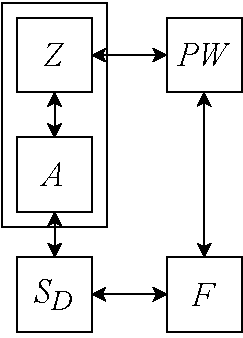
\includegraphics[scale=0.5]{figures/dummylemma_pre.pdf}
	\caption{An environment running \A internally is captured by the $\forall$ quantifier for the emulation definition with respect to the dummy adversary.}
	\label{fig:dummy_pre}
	\end{subfigure}
	~
	\begin{subfigure}[t]{0.2\textwidth}
	\centering
	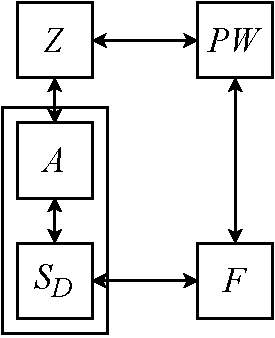
\includegraphics[scale=0.5]{figures/dummylemma_post.pdf}
	\caption{Moving the adverary out of \Z and into the execution results in the same inputs to the protocol and functionalities in both worlds and hence we expect emulation to hold.}
	\label{fig:dummy_post}
	\end{subfigure}
	\caption{Graphical illustration of the intuition behind the Dummy Lemma.}
	\label{fig:dummylemmas}
\end{figure}


We restate the Dummy Lemma here:
\begin{theorem}[Dummy Lemma]\label{thm:dummy}
If \ $\exists \DS$ s.t. $ \DA, \DS \vdash \F_2 \xrightarrow{\pi} \F_1$ then $\forall \A \ \exists \Sim_\A$ s.t. $\Sim_{\A} \vdash  \F_2 \xrightarrow{\pi} \F_1)$ 
\end{theorem}

\begin{proof}
The constructed simulator $\Sim_\A$ runs \A and \DS internally.
$\Sim_\A$ sandboxes the two simulators using our virtual tokens construction.
The construction simulator is straightforward, and we provide sample snippets of code from the simulator.
The adversaries \A and \DS expect to receive input from \Z through communicator.

The simulator creates channels for each of \A and \DS and connects them together.
For example, output from \A on its channel to a party or the functionality is merged 
into input from \Z for \DS.
In the dummy simulator the channels are created as:
\begin{lstlisting}[basicstyle=\footnotesize\BeraMonottFamily, frame=single,  mathescape]
#a2ps <- channel_init[K1][p2f] ;
#a2fs <- channel_init[K1][s2f] ;
#z2s <- channl_init[K1][Z2A[p2f][s2f]] ;
<- a2z_wrap[K][p2f][s2f] <- #a2ps #a2fs #z2s ;
\end{lstlisting}
where \inline{a2z_wrap} simply reads from \inline{#a2ps} and \inline{#a2fs} and wraps it in the type constructor for messages from \Z to \A:
\begin{lstlisting}[basicstyle=\footnotesize\BeraMonottFamily, frame=single,  mathescape]
$\nproc$ a2s_wrap[K][a][b]:
  (#in2p: comm[K][a]), (#in2f: comm[K][b]), 
  (#out: comm[K][Z2A[a][b]) |- ($\$$c : 1) =
{
  $\nmatch$ #in2p, #in2f (
    *,m => #out.SEND ; $\nsend$ #out Z2A2F(m) ;
    A2P(pid,m),* => #out.SEND ; 
    $\nsend$ #out Z2A2P(pid, m) ;
  )
  $\$$c <- a2s_wrap[K][a][b] <- #in2p #in2f #out 
}
\end{lstlisting}

On input from \Z, we simply forward the message with virtual tokens instead of real tokens and outgoing messages from \A as real output to \Z:
\begin{lstlisting}[basicstyle=\footnotesize\BeraMonottFamily, frame=single,  mathescape]
$\nmatch$ #z2a {z2an} K, #a2z' {a2zn} K1 (
  m,* =>
    $\nwithdraw$ K K1 {z2an} ;
    #z2a'.SEND; $\nsend$ #z2a' pid ; $\nsend$ #z2a' m ;
    $\npay$ K1 {z2an} #z2a' ;
  *,m =>
    #z2a'.SEND; $\nsend$ #z2a' pid ; $\nsend$ #z2a' m ;
    $\npay$ K {z2an} #z2a' ;
)
\end{lstlisting}
We use the \inline{match} over shared channels as syntax sugar that abstracts away their special handling and receiving the given import and token type from them. 

Input from the ideal world \F or the \partywrapper is forwarded, virtualy, to \DS in the same way as above. 
\end{proof}
